\documentclass{beamer}
\usepackage[T1]{fontenc}
\usepackage[utf8]{inputenc}
\usepackage{lmodern}
\usepackage{textcomp}
\usepackage{lastpage}
%
\title{Towards Socially Responsible AI: Cognitive Bias-Aware Multi-Objective Learning
}
%
\begin{document}
\normalsize
\maketitle
%
\begin{frame}{Introduction}
%
\begin{itemize}
\item
abd
\item
def
\item
ghi
\item
jkl
\end{itemize}
\end{frame}
%
\begin{frame}{Introduction}
%
\begin{figure}[t]
    \centering
    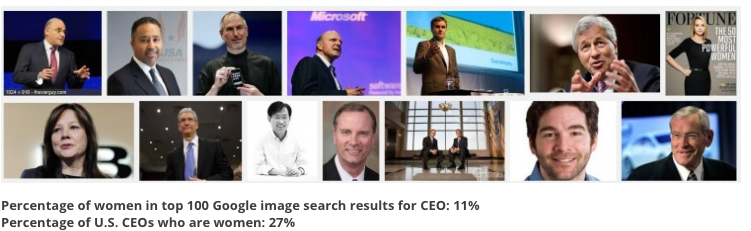
\includegraphics[width=.75\columnwidth]{ceo.png}
    
\includegraphics[width=.24\columnwidth]{qc.png}
    \caption{Examples of social bias in existing AI systems: `Google Image Search' under-representing women as CEOs (left), and `Google query completion' prioritizing \emph{appearance} over \emph{filmography} for a popular female actor (right).}
    \label{fig:bias-in-existing-AI-tools}
\end{figure}
\end{frame}
%
\begin{frame}{Related Work}
%
\begin{itemize}
\item
abd
\item
def
\item
ghi
\item
jkl
\end{itemize}
\end{frame}
%
\begin{frame}{Bias-Aware Predictions}
%
\begin{itemize}
\item
abd
\item
def
\item
ghi
\item
jkl
\end{itemize}
\end{frame}
%
\begin{frame}{Bias-Aware Predictions}
%
\begin{figure}[t]
    \centering
    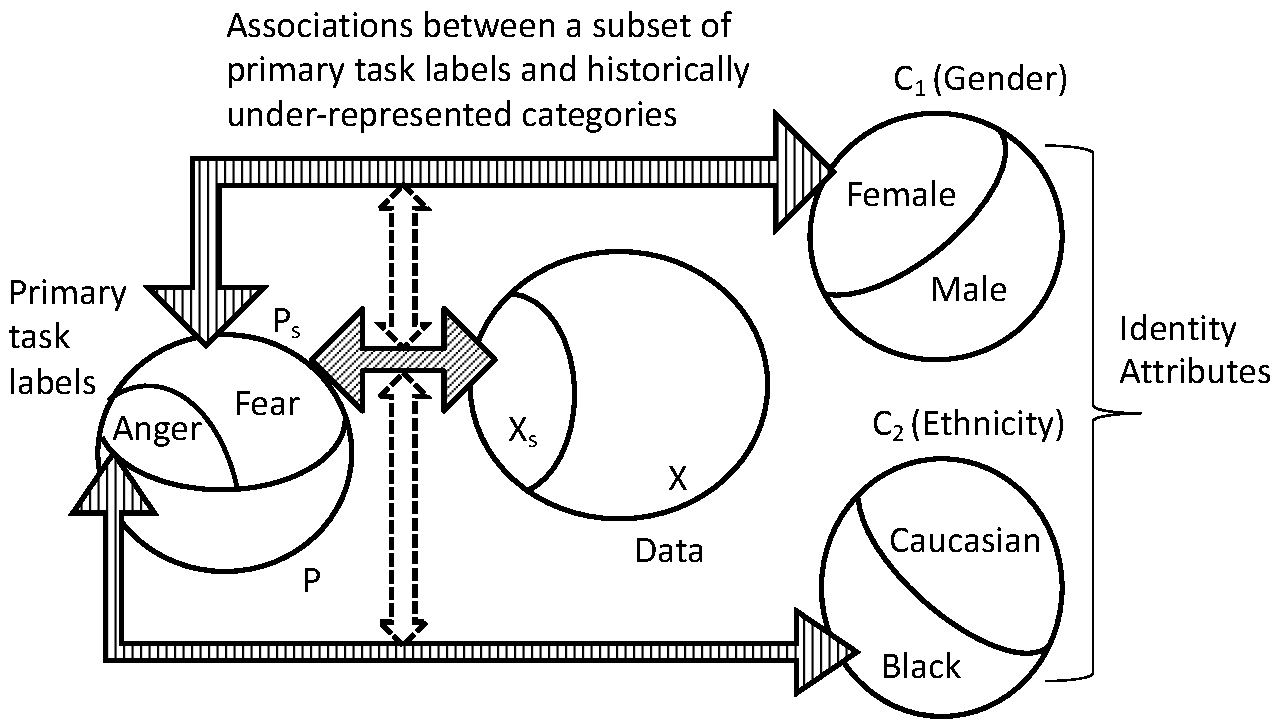
\includegraphics[width=.8\columnwidth]{bias-schematic.pdf}
    \caption{Schematic of cognitive bias removal.}
    \label{fig:schematic-bias}
\end{figure}
\end{frame}
%
\begin{frame}{Bias-Aware Predictions}
%
\begin{figure}[t]
    \centering
    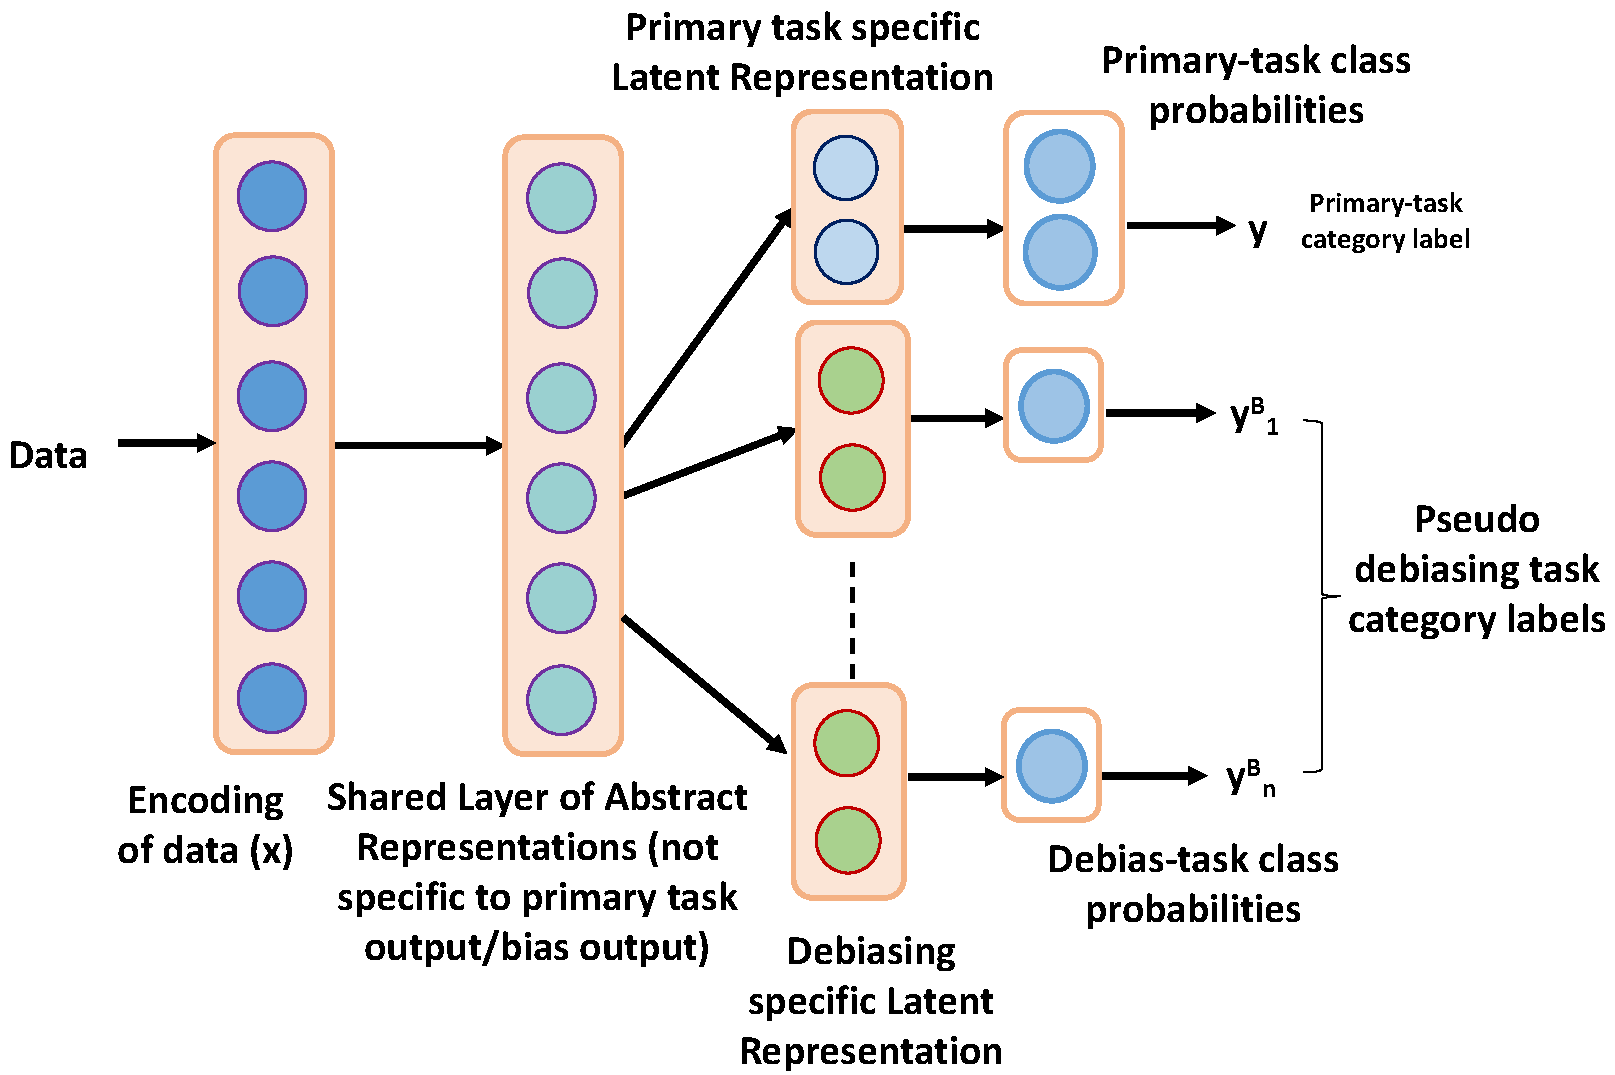
\includegraphics[width=.85\columnwidth]{debias-architecture.pdf}
    \caption{Schematic diagram of a neural network architecture for \emph{jointly} learning the primary task objective (for effective prediction) and a set of debiasing tasks (for reducing the cognitive bias in these predictions).}
\label{fig:deBiasArch}
\end{figure}
\end{frame}
%
\begin{frame}{Bias-Aware Predictions}
%
\begin{table}[t]
    \centering
    \small
    \begin{tabularx}{\columnwidth}{@{}l@{~~}X@{}}
    \toprule
    $\{(\vec{x}, y(\vec{x}))\}_{j=1}^{M}$ & $M$ pairs of data and primary task labels \\
    $P \in \{0,\ldots,k\}$ & Primary task label categories \\ 
    $P_s \in \{0,\ldots,k_s\}$ & A subset of $k_s (< k)$ categories, (e.g. `fear') \\
    $n$ & \#identity attributes (e.g. `gender') \\
    $z_i$ & Categorical variable for the \ith identity attribute with $m_i$ possible values \\
    $C_i=\{0,\ldots,m_i\}$ & Set of categories of the \ith identity attribute (e.g. `male', `female') \\
    $U_i \subset C_i$ & A set of (historically) under-represented categories, e.g. `female' \\
    $D_i \subset C_i$ & Historically dominating categories, e.g. `male'
    \\
    $Y^B_i \in \{0,1\}$ & Indicator variables for learning the pseudo-task of generating biased responses.\\
    \bottomrule
    \end{tabularx}
    \caption{Summary of notations.}
    \label{tab:notations}
\end{table}
\end{frame}
%
\begin{frame}{Bias-Aware Predictions}
%
\begin{equation}
X=\{(\vecxj, y(\vecxj)\}_{j=1}^{M}, \vecxj \in \mathbb{R}^d,
y(\vecxj) \in P=\{0,\ldots,k\}
\end{equation}
\end{frame}
%
\begin{frame}{Bias-Aware Predictions}
%
\begin{equation}
\phi: (\vec{x},\y(\vec{x})) \mapsto \Delta_{k},\,\, \vec{x} \in X \label{eq:primary-transformation},    
\end{equation}
\end{frame}
%
\begin{frame}{Bias-Aware Predictions}
%
\begin{equation}
y^B_i(\vec{x}) =
\begin{cases} 
1, & \frac{\mathbb{I}(y(\vec{x}) \in P_s \land z_i \in U_i)}{\mathbb{I}(y(\vec{x}) \in P_s)} > \tau\\
0, & \mathrm{otherwise}  \label{eq:yb-def}
\end{cases}
\end{equation}
\end{frame}
%
\begin{frame}{Bias-Aware Predictions}
%
\begin{equation}
\phi^B_i: (\vec{x}, y^B_i) \mapsto \Delta_{1},\,\, \vec{x} \in X_s = \{\vec{x}: y(\vec{x}) \in P_s\}.  \label{eq:biastaskmap}
\end{equation}
\end{frame}
%
\begin{frame}{Bias-Aware Predictions}
%
\begin{equation}
\begin{split}
\hat{y} & = \mathrm{softmax}(\Theta_p(\Theta_s(\vec{x}))), \Theta_p \in \mathbb{R}^{p \times k} \\
\hat{y^B_i} & = \mathrm{sigmoid}(\Theta^B_i(\Theta_s(\vec{x}))), \Theta^B_{i} \in \mathbb{R}^{p \times 1}, \vec{x} \in X_s \label{eq:softmax}.
\end{split}
\end{equation}
\end{frame}
%
\begin{frame}{Bias-Aware Predictions}
%
\begin{equation}
\mathcal{L}=P(y|\vec{x};\Theta_p,\Theta_s) - \sum_{i=1}^{n} P(y^B_i|\vec{x};\Theta^B_{i},\Theta_s), \label{eq:jointloss}
\end{equation}
\end{frame}
%
\begin{frame}{Evaluation}
%
\begin{itemize}
\item
abd
\item
def
\item
ghi
\item
jkl
\end{itemize}
\end{frame}
%
\begin{frame}{Evaluation}
%
\begin{figure}[t]
\centering
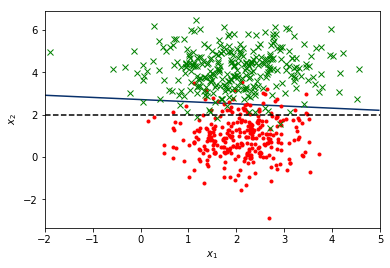
\includegraphics[width=0.49\columnwidth]{biased_boundary.png}
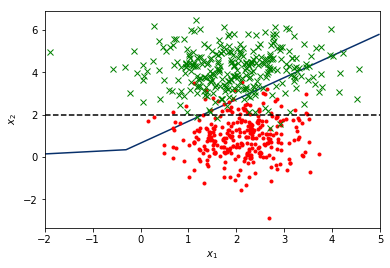
\includegraphics[width=0.49\columnwidth]{debiased_boundary.png}
\caption{Illustrative example to visualize bias reduction with multi-objective learning (Equation \ref{eq:jointloss}). Predictions
with a bias-agnostic classifier (logistic regression with $L_2$ regularization) are effective but exhibits a `bias' in associating the green points with the top half of the plot area (left); whereas the multi-objective learning is able to reduce such a bias (right).
\label{fig:2d-data}}
\end{figure}
\end{frame}
%
\begin{frame}{Evaluation}
%
\begin{table}[t]
\centering
\scriptsize
\begin{tabular}{l@{~~}c@{~~}c@{~~}c@{~~}c@{~~}c@{~~}c} 
\toprule
&\multicolumn{5}{c}{Emotion Categories}& \\
\cmidrule(r){2-6}
Identity Attribute &Fear & Anger & Joy & Sadness & Neutral & Total \\
\midrule
Male &1050&	1050&	1050 &	1050&	120	& 4320\\
Female &1050&	1050&	1050 &	1050&	120	& 4320\\
African-American  &700&	700	&700&	700&	120&	2920\\
Caucasian  &700&	700	&700&	700&	120&	2920\\
None  &N/A&	N/A	&N/A&	N/A&	2920 &	2920\\
\midrule
\midrule
\multicolumn{7}{c}{(SS-1): Biased Subsample with (Female, Fear)$\uparrow$, (Male, Anger)$\uparrow$} \\
\midrule
Male &500&	1050&	1050&	1050&	120&	3770\\
Female &1050&	500&	1050&	1050&	120	&3770\\
African-American &450	&550 &	700	&700&	120	&2520\\
Caucasian  &550&	500	&700&700&120&	2570\\
None  &N/A& N/A& N/A & N/A & 1450 & 1450 \\
\midrule
\midrule
\multicolumn{7}{c}{(SS-2): Biased Subsample with (Caucasian, Fear)$\uparrow$} \\
\midrule
Male &850&	1050&	1050&	1050&	120&	3770\\
Female &850&	1050&	1050&	1050&	120	&3770\\
African-American &300	&700 &	700	&700&	120	&2520\\
Caucasian  &700&	700	&700&700&120&	2570\\
None  &N/A& N/A& N/A & N/A & 1450 & 1450 \\
\bottomrule
\end{tabular}
\caption{Fear Distribution }
\label{tab:DataDesc}
\end{table}
\end{frame}
%
\begin{frame}{Evaluation}
%
\begin{equation}
U_{x_2}=\{(x_1,x_2) \in \mathbb{R}^2: x_2 > 2\} \label{eq:2dexample}
\end{equation}
\end{frame}
%
\begin{frame}{Evaluation}
%
\begin{equation}
F=\alpha(1-\alpha),\, \alpha=P(y=l|U),
\end{equation}
\end{frame}
%
\begin{frame}{Evaluation}
%
\begin{equation}
\gamma = \frac{AF}{A+F},    
\end{equation}
\end{frame}
%
\begin{frame}{Conclusions and Future Work}
%
\begin{itemize}
\item
abd
\item
def
\item
ghi
\item
jkl
\end{itemize}
\end{frame}
%
\begin{frame}{Conclusions and Future Work}
%
\begin{table}[t]
\footnotesize
\centering
\begin{tabular}{l|c|c|c|c|c|c|c}
\toprule
Method & $Obj$ & $JOBJ$ & Penalty & $Gender$  & Race & $Debiased_Embedding$  \\
\midrule
STWR & \checkmark & \checkmark  &  &  & & & \checkmark &  \\
QFG & \checkmark &   & \checkmark &  & & & & \checkmark \\
QFG + RLM & \checkmark & \checkmark  & \checkmark &  & & & \checkmark & \\
CRLM & \checkmark &   & \checkmark & \checkmark & &\checkmark &\checkmark &  \\
WE & \checkmark &   & \checkmark & \checkmark &\checkmark & &\checkmark &  \\
WET & \checkmark &   & \checkmark & \checkmark &\checkmark &\checkmark &\checkmark &  \\
D2V & \checkmark &   & \checkmark & \checkmark &\checkmark &\checkmark &\checkmark &  \checkmark\\
NMF & \checkmark &   & \checkmark & \checkmark &\checkmark &\checkmark &\checkmark &  \checkmark\\
GRL & \checkmark &   & \checkmark & \checkmark &\checkmark &\checkmark &\checkmark &  \checkmark\\
\bottomrule
\end{tabular}
\caption{A summary of the approaches investigated. The columns denote sources of information, e.g. representation learning (RL), temporal information (T), weighted query (WQ), joint representation (JRL).}
\label{tab:baselines}
\end{table}
\end{frame}
%
\end{document}
